% !TeX encoding = UTF-8
% !TeX spellcheck = en_GB
% !TeX root = mythesis.tex
\chapter{Wigner function of different shape pulses}

%The  Third appendix

\section{A sinus shape emitting one electron than one hole}

\subsection{Wigner}

\begin{figure}[hptb]
	\begin{center}
		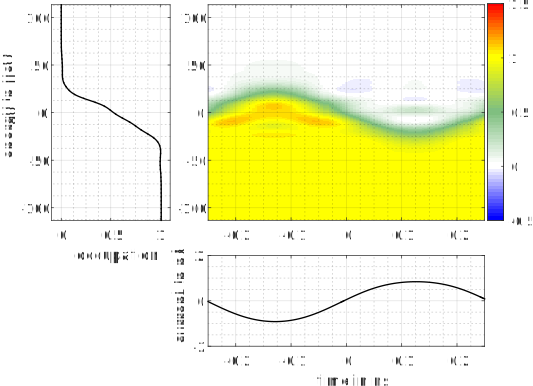
\includegraphics[width = 10 cm]{./appC/wigData_sinus_Projected_Gradient_Method} 
	\end{center}
	
	\caption{Wigner sinus}
	\label{fig: Wigner sinus}
\end{figure}

\subsection{Probabilities and Coherences}

\begin{figure}[hptb]
	\begin{center}
		\begin{tabular}{c c c c}
			(a) & & (b) & \\ 
			& \includegraphics[width = 6.5 cm]{./appC/JnlData_sinus_Projected_Gradient_Method_proba_el} & & 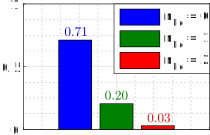
\includegraphics[width = 6.5 cm]{./appC/JnlData_sinus_Projected_Gradient_Method_proba_ho}
		\end{tabular}
	\end{center}
	
	\caption{proba sinus}
	\label{fig: proba sinus}
\end{figure}



\begin{figure}[hptb]
	\begin{center}
		\begin{tabular}{c c c c}
			(a) & & (b) & \\ 
			& 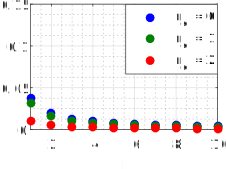
\includegraphics[width = 6.5 cm]{./appC/JnlData_sinus_Projected_Gradient_Method_coh_el_el} & & \includegraphics[width = 6.5 cm]{./appC/JnlData_sinus_Projected_Gradient_Method_coh_ho_ho} \\
			(c) & & & \\
			& \includegraphics[width = 6.5 cm]{./appC/JnlData_sinus_Projected_Gradient_Method_coh_el_ho} & & 
		\end{tabular}
	\end{center}
	
	\caption{coherence sinus}
	\label{fig: coherence sinus}
\end{figure}

\subsection{Wavefunctions}

\begin{figure}[hptb]
	\begin{center}
		\begin{tabular}{c c c c}
			(a) & & (b) & \\ 
			& 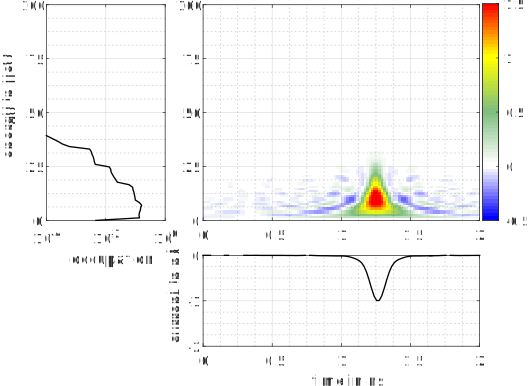
\includegraphics[width = 6.5 cm]{./appC/wannierwigData_sinus_Projected_Gradient_Method-el-0} & & 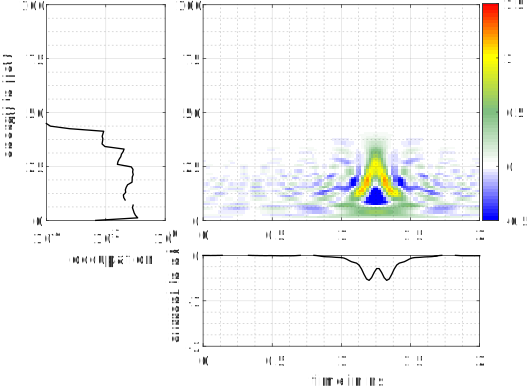
\includegraphics[width = 6.5 cm]{./appC/wannierwigData_sinus_Projected_Gradient_Method-el-1} \\
			(c) & & (d) & \\
			& 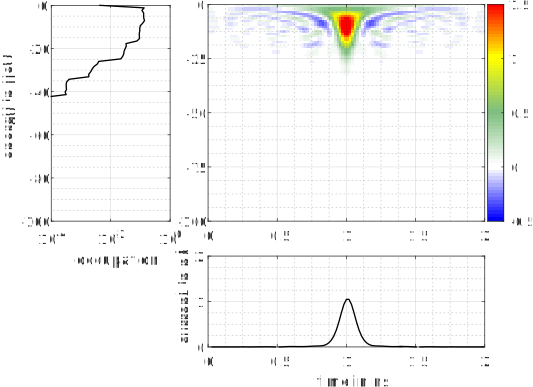
\includegraphics[width = 6.5 cm]{./appC/wannierwigData_sinus_Projected_Gradient_Method-ho-0} & & 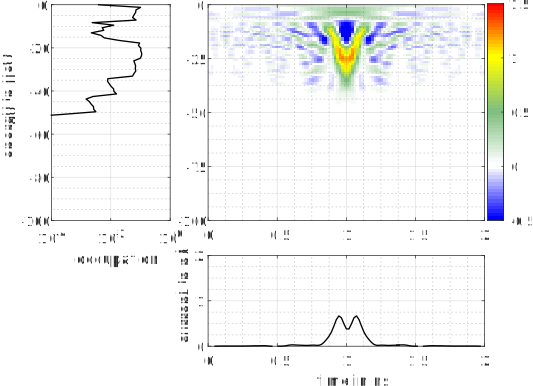
\includegraphics[width = 6.5 cm]{./appC/wannierwigData_sinus_Projected_Gradient_Method-ho-1}
		\end{tabular}
	\end{center}
	
	\caption{wannier sinus overlap après rotation de pi/2*0.38 de 0.95 avec des Levitons de largeur 80 ps}
	\label{fig: wannier sinus}
\end{figure}

\section{An asymmetric pulse with exponentially decreasing current \label{sec: An asymetric pulse with exponentially decreasing current}}

\subsection{Wigner}

\begin{figure}[hptb]
	\begin{center}
		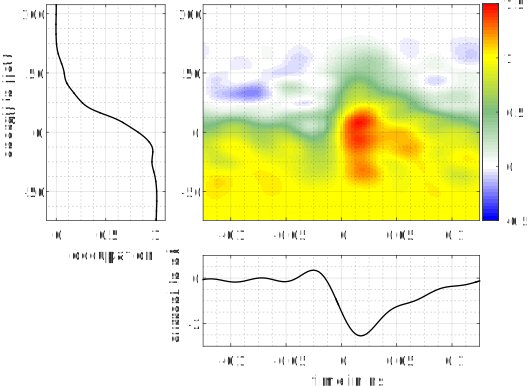
\includegraphics[width = 10 cm]{./appC/wigData_exponential_50ps_1e_JMAP_f_vf} 
	\end{center}
	
	\caption{Wigner exponential}
	\label{fig: Wigner exponential}
\end{figure}

\subsection{Probabilities and Coherences}

\begin{figure}[hptb]
	\begin{center}
		\begin{tabular}{c c c c}
			(a) & & &   \\ 
			& \includegraphics[width = 5cm]{./appC/JnlData_exponential_50ps_1e_JMAP_f_vf_proba} &
			&  \\
			(b) & & (c) & \\
			& 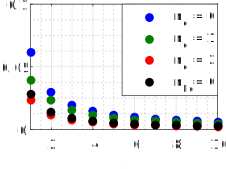
\includegraphics[width = 5cm]{./appC/JnlData_exponential_50ps_1e_JMAP_f_vf_coh_inter_period} &
			& 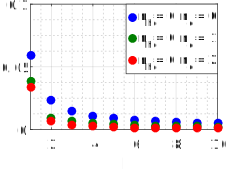
\includegraphics[width = 5cm]{./appC/JnlData_exponential_50ps_1e_JMAP_f_vf_coh_el_ho}
		\end{tabular} 
	\end{center}
	\caption{(a) pi du exponential (b) coh du exponential}
	\label{fig: Jnl exponantial}
\end{figure}

\subsection{Wavefunctions}

\begin{figure}[hptb]
	\begin{center}
		\begin{tabular}{c c c c}
			(a) & & (b) & \\ 
			& 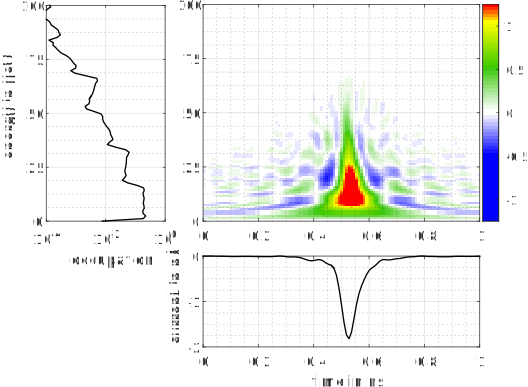
\includegraphics[width = 6.5 cm]{./appC/wannierwigData_exponential_50ps_1e_JMAP_f_vf-el-0} & & 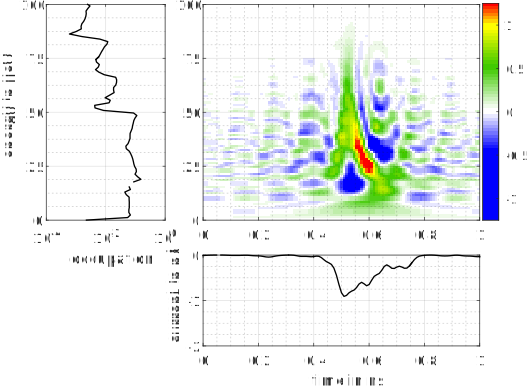
\includegraphics[width = 6.5 cm]{./appC/wannierwigData_exponential_50ps_1e_JMAP_f_vf-el-1} \\
			(c) & & & \\
			& 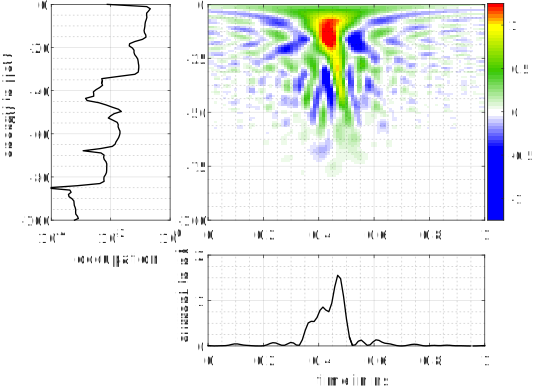
\includegraphics[width = 6.5 cm]{./appC/wannierwigData_exponential_50ps_1e_JMAP_f_vf-ho-0} & &
		\end{tabular}
	\end{center}
	
	\caption{wannier exponential}
	\label{fig: wannier exponential}
\end{figure}

\begin{figure}[hptb]
	\begin{center}
		\begin{tabular}{c c c c}
			(a) & & (b) & \\ 
			& 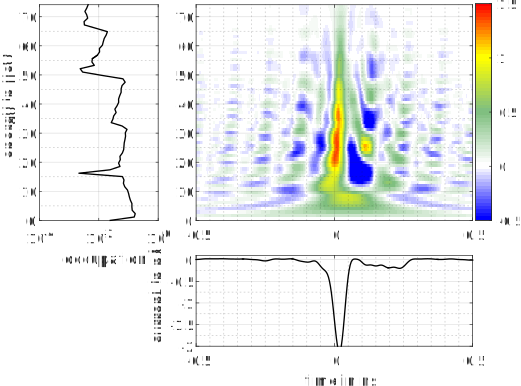
\includegraphics[width = 6.5 cm]{./appC/wannierwigData_exponential_50ps_1e_JMAP_f_vf-el-moins-y} & & 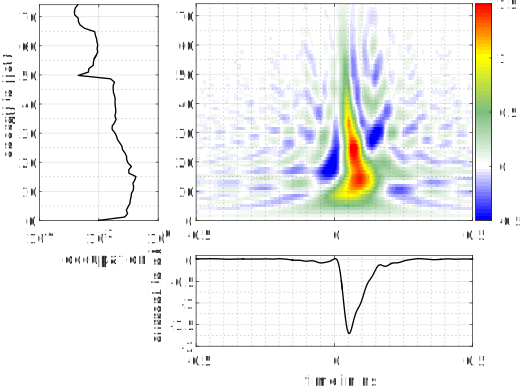
\includegraphics[width = 6.5 cm]{./appC/wannierwigData_exponential_50ps_1e_JMAP_f_vf-el-plus-y}
		\end{tabular}
	\end{center}
	
	\caption{y axis wannier exponential}
	\label{fig: y axis wannier exponential}
\end{figure}

